%!TEX root =  report.tex
\section{Semantic Gossip}
\label{sec:semantic}

%\new
In this section, we first motivate investigating the interplay between consensus protocols and gossip communication. We then propose semantic gossip mechanisms, and elaborate on design details.

% motivation - in the Tendermint case - 
% what are situations where Tendermint's and gossip's redundancy could be reduced ?  ...
% concrete situations where communication could be spared.   unneeded (motivate filtering), optimisations possible  (motivate aggregation)

% design -

% layering

% semantic filtering 

% semantic aggregation

% implementation

% motivate the need for gossip protocols optimized for consensus, 
% describe the design of a gossip protocol that takes advantage of consensus semantics, 
% and detail its implementation.



\subsection{Motivation}
\label{sec:motivation}

Using gossip as a communication layer for consensus is in general a straigthforward adaptation:
the direct point-to-point communication using a set of channels providing full connectivity
is replaced by gossip a layer that reaches all processes.  
%
One of the reasons it is straightforward is because the consensus layer deals with process failures and communication problems that may arise, which makes it robust  to be used with different underlying communication properties.    
%The Tendermint protocol uses gossip for interprocess communication.  

In the following we discuss two fundamental characteristics of a wide range of consensus protocols
that motivate the investigation of the interplay of consensus with a gossip communication layer.

\subsubsection{Detecting quorums}
\label{redundant}

%generic
One way to design redundant systems is through the concept of quorums.
A quourum can be understood as a level of redundancy sufficient to allow the protocol to progress while keeping safety, under the fault model assumption.    
%When a node gathered matching messages from a quorum of nodes, further messages belonging to the same step are typically ignored at the node, i.e. redundant.
%generic
Considering this, a node could spare to send messages if it already knows a quorum has been
achieved by other nodes.
While this observation does not help when nodes communicate directly,
%
%Using point-to-point communication this approach is not natural, if not impossible to explore since this would mean that a node would await a quourum to be built to spare sending a messsage that should contribute to that quorum - a contradiction.    
%
%However, 
the use of gossip at the communication level allows to benefit from it.  
If a node receives a message $m$ and computes that it already has matching messages from a quorum of nodes, it assumes the previous messages, sufficient to build a quorum, were forwarded.  Thus the redundant message $m$ (and further ones) is not needed at the neighbour nodes and is not forwarded.
This redundancy elimination is however only possible if the gossip layer is aware of the consensus protocol semantics.

\subsubsection{Phased communication}
\label{obsolete}
%generic
Consensus protocols are typically organized in communication instances, and proceed in rounds using corresponding message types.
This helps to detect if a given message is obsolete for the current progress of the protocol. %  It could have been delayed or originated by a late node, and is no longer valid. 
In such case it could be ignored.
%
A further observation is that,
as nodes behave simmetrically, 
it is common that the same types of messages, stemming from different nodes are communicated concurrently through the network.
%
While using direct communication this maybe a pointless observation,
when using gossip we can unfold the examination:
messages with the same semantics, but differing in the specific node's
answers (e.g. votes), will coexist in intermediate nodes along the gossip forwarding.
Moreover, it is typical that such messages are addressed to the same set of nodes (all that participate in the consensus protocol).  
In such cases, instead of forwarding and processing separately each such message, they can be aggregated at an intermediate node, 
resulting one message collecting the space of parameters of the equivalent bunch of messages.
This leads to sparing both messages through the network as also message processing at destinations. 

\old

\subsection{Design}
\label{sec:design}

In this section, we discuss simple techniques to address the mismatch between a
fault-tolerant consensus algorithm, using Tendermint as reference, and the
underlying gossip communication substrate.
The goal is to reduce the message redundancy at the gossip layer,
employing the knowledge about the message semantics provided by the
consensus algorithm.
The challenge is to achieve this reduction in message redundancy without sacrificing
(a) modularity, (b) consensus properties, and (c) the original resilience guarantees offered by gossip. 

\subsubsection{Semantic filtering}

The first technique allows the consensus algorithm to decide whether a message should be sent to other nodes at the gossip layer.
%This means interferring with the operation of the gossip layer, which, by default, forwards every message received.
The consensus algorithm can then restrain the propagation of messages that are (potentially) no longer useful to other nodes.
%The main goal is to save network and processing resources that would be used to forward messages that peers will probably disregard.
Semantic filtering is implemented through a set of rules to identify messages that, according to the consensus semantics, have become redundant or obsolete, as discussed in Sections \ref{redundant} and \ref{obsolete}.
%
The semantic filtering rules are evaluated when a message is ready to be sent to peer nodes.
If the message is filtered out, because it is identified as either obsolete or redundant, the gossip layer discards it; otherwise, it is sent as usual.

The evaluation of the semantic filtering rules can be seen as a lightweight
execution of the consensus algorithm on behalf of another node.
In fact, to identify messages that can be filtered out it is necessary to store
some information about messages that were previously sent to other nodes.
The more comprehensive the rules are, the more information is stored per peer node,
and the more costly it is to evaluate them.
Thus, the choice of a set of semantic filtering rules should balance the cost
of evaluating them for every message forwarded, with the benefits that an
effective filtering can provide.

\paragraph{Semantic filtering in Tendermint} 
As discussed  in Section \ref{sec:Tendermint}, a node progresses   to the next step when a quorum of \textsc{prevote} or \textsc{precommit} matching messages is received.  Additional messages of these types are not needed.  Also, duplicted messages are not usefull and need not to be forwarded.   The filtering rules thus state that a vote message is dropped by a node in the following cases:  
\begin{itemize}
\item If a vote of the same type (either \textsc{prevote} or \textsc{precommit}), with the same originator,  height, round, and value has been already computed before by the node;
\item If the vote (either \textsc{prevote} or \textsc{precommit}) is for a height and round for which the node has already handled a quorum of matching votes.
\end{itemize}

\paragraph{Semantic filtering keeps consensus properties}

Discarding messages at the gossip level is perceived as message loss (absence of) at the consensus level.  Thus, filtering could at most prevent progress but not safety.
To ensure progress, a filtering mechanism cannot hinder nodes from receiving messages from a quorum. 
%
Notice that with the first filtering rule the message dropped has been handled before and
with the second filtering rule, a node discards messages after having handled a quorum of matching messages.   In both cases, since the node handled the previous messages, they were already forwarded via gossip to other nodes.  

\fp{The text here is unclear, as the message already could be lost.}

\fp{What does it mean for ``a quoru to be identified at a node''?}  

%In such case, the node already forwarded a quorum of messages to its neighbours that, therefore, already have votes to build a quorum too. Again, the current message is not needed.

\subsubsection{Semantic aggregation}

The second technique provides the consensus algorithm with the possibility to
replace a number of similar or related messages, which will be sent to a peer,
with a single message comprising the information carried by the original
messages.
This technique explores the scenario in which the gossip layer has multiple
pending messages to send to a peer, so that some of them are likely, according
with the consensus semantics, to be aggregated.
It is an opportunistic mechanism that aims to reduce the number of messages
exchanged by processes via gossip, especially when they operate under moderate
to high load.

Semantic aggregation is also implemented through a set of rules that, from a
list of pending messages: (i) identify those that are prone to aggregation, and
(ii) define how an aggregated message can be built from the original messages.
When messages prone to aggregation are found, the first of them in the list of
pending messages is replaced by the aggregated message, built according to
the respective rule, while the remaining ones are removed from the list.
In other words, an aggregated message both replaces and filters out the
original messages that it aggregates.
Messages that are not prone to aggregation, or for which aggregation is not
deemed advantageous by the consensus algorithm, are not affected by this
technique.
They are kept in the list of pending messages, and are forwarded to the peers as
usual.

Semantic aggregation rules can be either reversible or not.
When a process receives from a peer a message aggregated using a reversible
rule, it reconstructs the original messages and treats them as regular messages.
That is, messages received for the first time are delivered to the
consensus algorithm and forwarded to other peers.
In this process, in
particular, they can be semantically aggregated again.
When an aggregated message is built from a non-reversible rule, it is treated
as a new message broadcast by the process that aggregated it.
In this case, the consensus algorithm must be able to handle the
semantically aggregated message.

Observe that, despite the similarities, semantic aggregation is not the same as
batching~\cite{FR95}.
When implemented at network level, batching essentially concatenates messages,
treated as raw byte arrays, to optimize the network usage.
At application level, some message types are batched until the batch size
reaches a threshold or a timeout expires.
As a result, batching can have negative effect on performance when the system
is subject to low loads, as the sending of messages is postponed.
This does not happen with semantic aggregation, which despite being ineffective
under low loads, does not delay the sending of any messages.
Moreover, the technique is more flexible than batching, as messages are not
only concatenated, but can be transformed, merged, in any arbitrary way defined
by semantic aggregation rules.

\paragraph{Semantic aggregation in Tendermint}

Regarding Tendermint, semantic aggregation is also applied to 
\textsc{prevote} and \textsc{precommit} voting messages.
Given a subset of messages to be sent to a peer, messages of the same type (\textsc{prevote} or \textsc{precommit}), for the same height, round and value (block id) can be aggregated.
The aggregated message carries a list of pairs $\langle origin, signature \rangle$ identifying originators of the  messages aggregated, and only once the identical contents.

\paragraph{Semantic aggregation keeps consensus properties}

The basic requirement for a sound aggregation strategy is that the information conveyed by an aggregated message is equivalent to the original non-aggregated ones, enabling the same decisions to be taken at the destination.
%
%Observe that the aggregation rule proposed for Tendermint does not exclude information, only data.\fp{I don't get this. What's the difference between information and data?}

Notice that the restriction to aggregation is strong: aggregated messages should be identical, only stemming from different originators.   
%
The receiver of the aggregated message, be it \textsc{prevote} or \textsc{precommit}, will compute the exact same votes as for the non-aggregated messages.
%
%A strong aggregation restriction makes it easier to show sound and, although it may seem less effective, as consensus protocols often use communication phases with same message types sent among processes, aggregation shows important benefits, as discussed further in the paper.\fp{Convoluted sentence...}

\subsubsection{Semantic Gossip and BFT}

To ensure that aggregation and filtering are not exploited by dishonest nodes,\footnote{For example, a dishonest node could forge messages to exploit the proposed mechanisms.  Consider a dishonest node $dh$ that forges a \textsc{prevote} message for a given height and round, pretending to be node $a$, and sends it to node $b$.  Since gossip does not verify messages, $b$ would record $dh$'s message and on the occasion of the original message from $a$, it would be filtered out with the effect of possibly preventing progress.} 
we ensure that any message is verified before the respective decisions are made by Semantic Gossip. \fp{I don't get this part.}




From an engineering perspective, as signature verification is one of the first measures taken at the consensus layer to avoid attacks, and being a costly procedure, instead of performing verification additionally at the gossip layer we propose an interface to return a copy of delivered and verified messages to the gossip layer.   With this, gossip can further handle the message without increasing the overall overhead.
This aspect is shown in Figure \ref{fig:architecture_sg} with the loop-back arch from signature verification at consensus to the filtering input queue at the semantic gossip layer.

%\fd{argue this is enough to handle bizantine processes ?}

%Semantic Gossip adopts that  Filtering and Aggregation decisions should be taken also based on verified messages.  


\subsection{Implementation}
\label{sec:impl}

%\color{violet}

We implemented a gossip-based communication layer to interconnect processes.
At the system setup, each process opens connections to a randomly selected set
of processes.  The resulting overlay has to be connected and each node is required to have at least $k=f+1$ neighbours.
Section \ref{sec:topos} discusses how nodes can create such an overlay using a distributed procedure.


\subsubsection{Classic gossip}

Figure~\ref{fig:architecture} (left) illustrates the architecture of a gossip layer.
A process interacts with the gossip layer through primitives {\em broadcast} and {\em deliver}.   Broadcast messages are handled just as gossip messages received from other peers.   Messages are delivered once they pass the duplication check.
The {\em delivery queue} offers messages to the upper layer.

A process also maintains, for each peer it is connected to, a Send and a
Receive routine. A {\em send queue} is associated to each Send routine; messages added to a {\em send queue} are eventually sent to the corresponding peer.
%There is a single {\em  receive queue} shared by 
All Receive routines share the same queue with the local broadcast.  
%
A message added to the {\em broadcast and delivered queues} is locally delivered and sent to
all peers but the peer the message came from: it is added to the {\em delivery
queue} and to all, but the message's origin, {\em send queue}s.
%
The selection of peers to which a message is sent is done by the message
forwarding module from the gossip main routine.    

%% Controlling the flood via recently seen cache
Messages are propagated using the {\em push} disseminating strategy. 
This means that the same message can be received by a
process several times, from distinct peers.
%
We control the flooding of messages using a simple approach based on a cache of recently received messages, maintained by every process.
%
A message is registered to the recently received cache before it is delivered
to the consensus algorithm and sent to the process' peers.
If the same message is received within a short period of time, so that the message's
identifier is still on the recently received cache, the message is
dropped---i.e., it is not delivered nor forwarded to the peers.
%
This is the role of the duplication check module represented in
Figure~\ref{fig:architecture}: it prevents, with some probability, a message
from being delivered and forwarded more than once. 
%
There is no actual guarantee of a deliver-and-forward once behavior, but the
adoption of a reasonable cache size reduces the probability
of message duplication.
%
It is worth noting that the cache stores message identifiers (hashes), not full messages, and so, it is relatively small.

\subsubsection{Semantic extensions}

The gossip layer offers two ways to control its behavior: semantic filtering and semantic aggregation, as presented in Section~\ref{sec:design}.
The consensus algorithm can adopt one or both techniques by implementing interface methods offered by the gossip layer.   
Figure \ref{fig:architecture_sg} (right) depicts how the classic gossip architecture is extended for filtering and aggregation, and identifies which functions are needed from the consensus layer, i.e., encapsulating semantics of the specific consensus protocol.

\begin{figure*}[htbp]
    \centering
    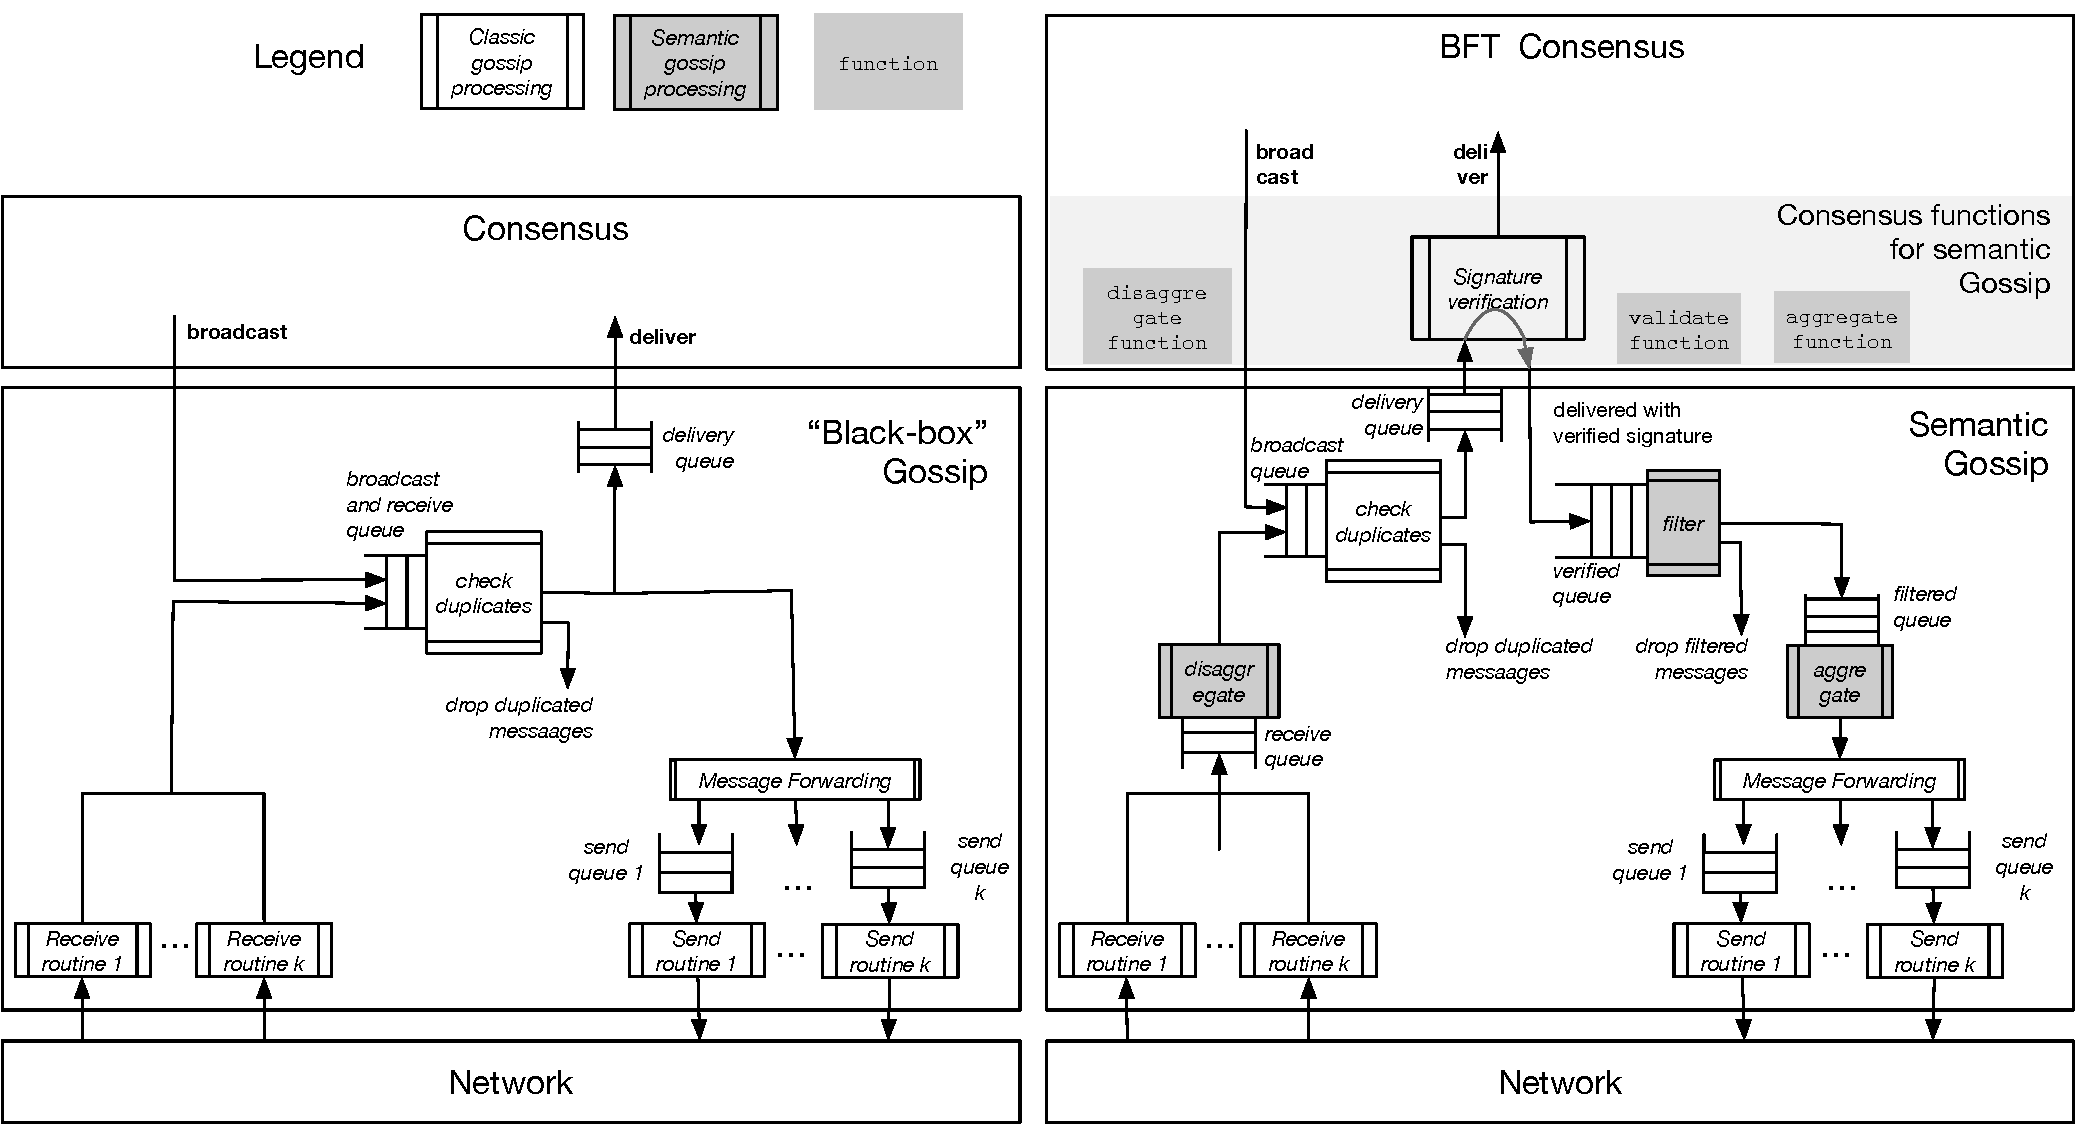
\includegraphics[width=1\columnwidth]{figures/architecture_SG3.pdf}

    
    \caption{Architectures: (left) - Gossip;  (right) Semantic Gossip}
    \label{fig:architecture}
    \label{fig:architecture_sg}
\vspace{-2mm}
\end{figure*}
% \begin{figure}[htbp]
%     \centering
%     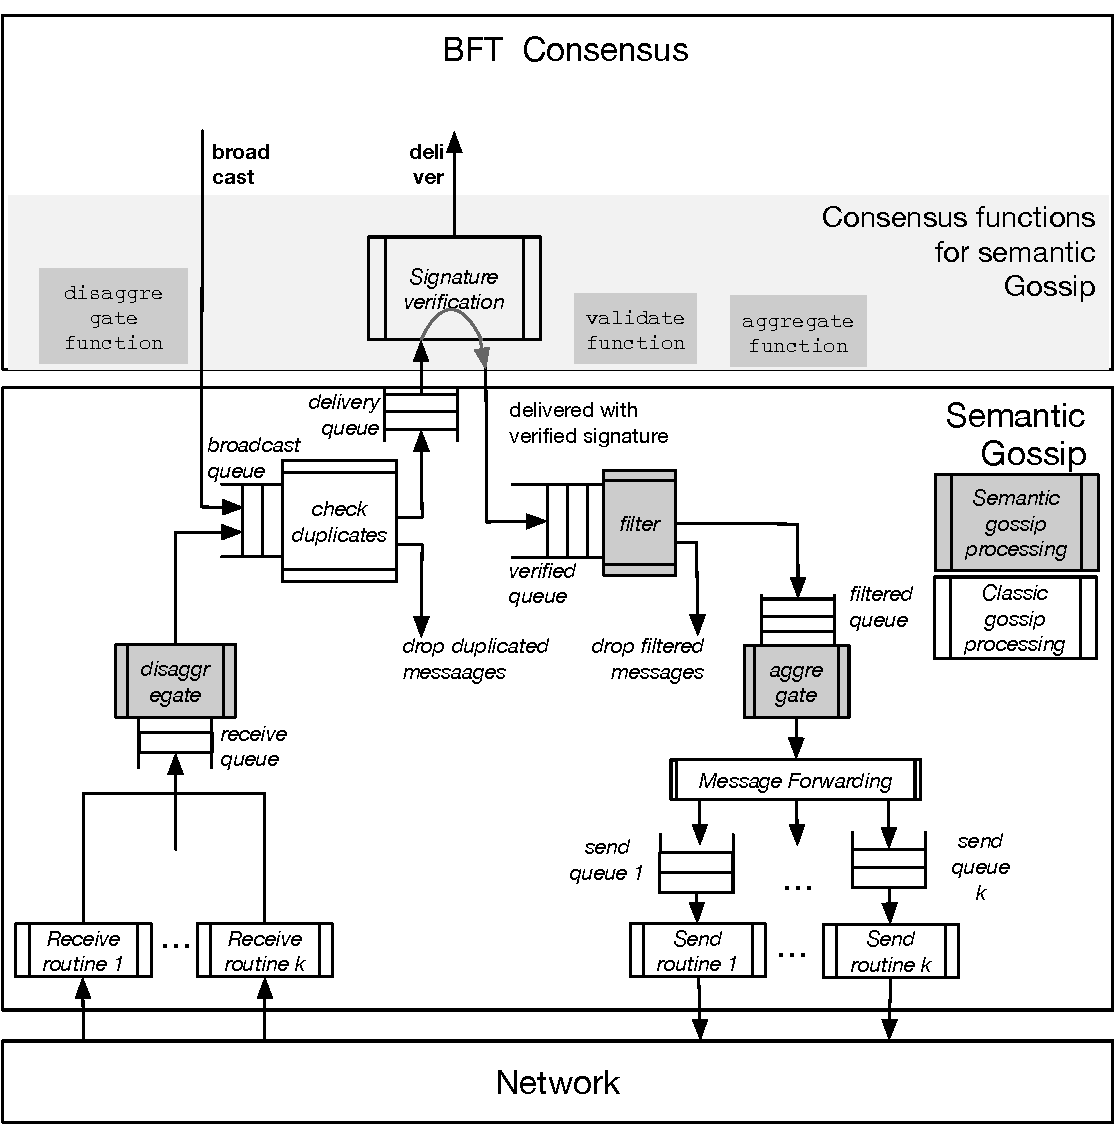
\includegraphics[width=1\columnwidth]{figures/architecture_SG2.pdf}
%     \caption{Architecture of semantic gossip at a process.}

% \end{figure}

\paragraph{Semantic filtering} is provided by allowing the consensus algorithm to implement
a {\em validate} function, which receives a message and a destination peer, and
returns a boolean:

\begin{verbatim}
Bool validate(Message, Peer)
\end{verbatim}
The {\em validate} function is invoked by the {\em filter} module at the gossip layer when a message has not been dropped due to duplicates or signature violation, and is considered for forwarding.
%
If the function returns false, the message is dropped, as the decision was to
filter out the message.
Otherwise, the message is sent to the peer, the default behavior when the
function is not implemented.
%
Implementations of the {\em validate} function should be fast and non-blocking,
as it is likely to be invoked concurrently by multiple sending routines.
The implementation should keep some information about the state of each peer,
essentially a summary of relevant messages that were previously processed and
not filtered out, and thus sent to that peer.
The cost of storing such information versus the benefit in terms of resources
saving by filtering out messages that would be sent to a peer
should be considered.


\paragraph{Semantic aggregation} is provided through the implementation of a pair of
functions, {\em aggregate} and {\em disaggregate}, by the consensus layer:

\begin{verbatim}
Message[] aggregate(Message[], Peer)
Message[] disaggregate(Message)
\end{verbatim}

The {\em aggregate} function receives an array of messages and a destination
peer, and returns an array of messages.
It is invoked by the gossip {\em aggregate} module when there are multiple pending messages to be sent to the respective peer.
%
%\fd{AGGRETATION APPLIES TO DIFFERENT KINDS OF MESSAGES, TO THE SAME DESTINATION ?  OR ALL CONSTITUTENS OF AN AGGREGATED MESSAGE ARE OF THE SAME TYPE?}
%
Messages returned by the {\em aggregate} method, either original untouched or 
aggregated, are sent to the peer, in the order in which they are returned.

Any message received from peers can be aggregated.  
The {\em disaggregate} module at the gossip layer invokes the 
the {\em disaggregate} function provided by the consensus layer when a message marked as
aggregated is received.
The {\em disaggregate} function 
is the inverse of {\em aggregate}: it receives an aggregated message and returns an array of reconstructed messages, for reversible semantically aggregated
messages.
Messages returned by the method are processed as regular messages, in the order
in which they are returned.
These messages are checked against the recently received
cache and, if not duplicated, delivered and forwarded to peers.


